\documentclass[12pt,a4paper]{article}
\usepackage[utf8]{vietnam}
\usepackage{amsmath,amssymb}
\usepackage{tabularx}
\usepackage{tikz}
\usetikzlibrary{calc,angles,quotes,arrows.meta,patterns}
\usepackage{xcolor}
\usepackage{enumitem}
\usepackage{fancyhdr}
\usepackage[top=1.2cm, bottom=1.2cm, left=1.5cm, right=1.5cm]{geometry}
\usepackage[loigiai]{ex_test}
\SAOPTN{widthSA=2.8,heightSA=0.62}

\setlength{\headheight}{15pt}
\setlength{\parskip}{0pt}

\pagestyle{fancy}
\fancyhf{}
\rhead{\textit{Môn Toán 6 -- Hướng dẫn giải Đề số 7}}
\lhead{\textit{Bộ đề ôn tập Giữa học kì I}}
\cfoot{\thepage}

\begin{document}

\begin{center}
  \textbf{\Large HƯỚNG DẪN GIẢI CHI TIẾT VÀ BẢNG ĐÁP ÁN}\\
  \textbf{\large ĐỀ ÔN TẬP GIỮA HỌC KỲ I -- ĐỀ SỐ 7}\\
  \textit{Môn: Toán 6 -- Năm học 2026 -- 2027}
\end{center}
\vspace{2mm}

% --- BẢNG ĐÁP ÁN TRẮC NGHIỆM TÓM TẮT ---
\noindent\textbf{\large A. BẢNG ĐÁP ÁN TRẮC NGHIỆM TỔNG HỢP}
\vspace{1.5mm}

\noindent\textbf{1. Phần I (Mỗi câu trả lời đúng được 0,25 điểm):}
\begin{center}
\begin{tabular}{|c|c|c|c|c|c|c|c|c|c|c|c|c|}
\hline
\textbf{Câu} & \textbf{1} & \textbf{2} & \textbf{3} & \textbf{4} & \textbf{5} & \textbf{6} & \textbf{7} & \textbf{8} & \textbf{9} & \textbf{10} & \textbf{11} & \textbf{12} \\
\hline
\textbf{Đ/A} & \textbf{D} & \textbf{B} & \textbf{C} & \textbf{D} & \textbf{B} & \textbf{C} & \textbf{C} & \textbf{A} & \textbf{C} & \textbf{D} & \textbf{B} & \textbf{A} \\
\hline
\end{tabular}
\end{center}
\vspace{1mm}

\noindent\textbf{2. Phần II (Đúng 1 ý: 0,1đ; 2 ý: 0,25đ; 3 ý: 0,5đ; 4 ý: 1,0đ):}
\begin{center}
\begin{tabular}{|c|c|c|c|c||c|c|c|c|c|}
\hline
\textbf{Câu} & \textbf{a)} & \textbf{b)} & \textbf{c)} & \textbf{d)} & \textbf{Câu} & \textbf{a)} & \textbf{b)} & \textbf{c)} & \textbf{d)} \\
\hline
\textbf{Câu 1} & \textbf{S} & \textbf{S} & \textbf{Đ} & \textbf{Đ} & \textbf{Câu 2} & \textbf{S} & \textbf{Đ} & \textbf{S} & \textbf{Đ} \\
\hline
\end{tabular}
\end{center}
\vspace{1mm}

\noindent\textbf{3. Phần III (Mỗi câu trả lời đúng được 1,0 điểm):}
\begin{center}
\begin{tabular}{|c|c|c|}
\hline
\textbf{Câu} & \textbf{Câu 1} & \textbf{Câu 2} \\
\hline
\textbf{Đáp án} & \textbf{$x = 2; y = 0$} & \textbf{40} \\
\hline
\end{tabular}
\end{center}
\vspace{3mm}

% --- B. LỜI GIẢI CHI TIẾT ---
\noindent\textbf{\large B. LỜI GIẢI CHI TIẾT CÁC CÂU HỎI}
\vspace{2mm}

\noindent\textbf{\large PHẦN I. CÂU TRẮC NGHIỆM NHIỀU PHƯƠNG ÁN LỰA CHỌN}
\vspace{1mm}
\begin{ex}
Viết tập hợp các chữ số của số $2025$?
\choice
{$\{2; 0; 2; 5\}$}
{$\{2; 2; 5\}$}
{$\{2; 0; 2\}$}
{\True $\{0; 2; 5\}$}
\loigiai{
Số $2025$ gồm các chữ số 2, 0, 5. Trong một tập hợp, mỗi phần tử chỉ được viết một lần. Do đó, tập hợp các chữ số là $\{0; 2; 5\}$.
}
\end{ex}

\begin{ex}
Hãy so sánh hai số tự nhiên $n = 52\,136\,001$ và $m = 52\,135\,998$:
\choice
{$n = m$}
{\True $n > m$}
{$n < m$}
{$n \le m$}
\loigiai{
So sánh hai số từ hàng cao nhất đến hàng thấp nhất:\\Hai số có cùng các chữ số ở hàng chục triệu, hàng triệu, hàng trăm nghìn và hàng chục nghìn. Ở hàng nghìn, ta có $6 > 5$. Do đó $n > m$.
}
\end{ex}

\begin{ex}
Tính vận tốc của một ô tô biết rằng trong $6$ giờ ô tô đi được $324\text{ km}$:
\choice
{$48\text{ km/h}$}
{$51\text{ km/h}$}
{\True $54\text{ km/h}$}
{$57\text{ km/h}$}
\loigiai{
Vận tốc của ô tô là: $v = 324 : 6 = 54\text{ (km/h)}$.
}
\end{ex}

\begin{ex}
Cho hình bình hành có độ dài hai cạnh là $a, b$ và chiều cao tương ứng với cạnh đáy $a$ là $h$. Công thức tính diện tích của hình bình hành là:
\begin{center}
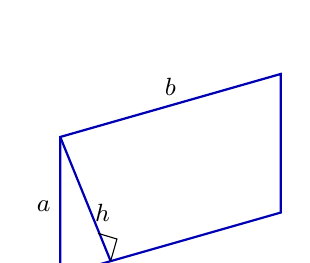
\begin{tikzpicture}[scale=0.8, font=\small]
  \coordinate (A) at (0,2.2);
  \coordinate (B) at (3.5,3.2);
  \coordinate (C) at (3.5,1);
  \coordinate (D) at (0,0);
  \draw[thick, blue!70!black] (A) -- (B) -- (C) -- (D) -- cycle;
  \draw[thick, blue!70!black] (A) -- (0.8,0.23) coordinate (H);
  \draw (0.8,0.23) -- (0.9,0.58) -- (0.6,0.67);
  \node[above] at (1.75,2.7) {$b$};
  \node[left] at (0,1.1) {$a$};
  \node[right] at (0.4,1) {$h$};
\end{tikzpicture}
\end{center}
\choice
{$S = a \cdot b$}
{$S = \dfrac{1}{2} a \cdot h$}
{$S = \dfrac{1}{2} b \cdot h$}
{\True $S = a \cdot h$}
\loigiai{
Diện tích hình bình hành bằng độ dài cạnh đáy nhân với chiều cao tương ứng. Ở đây, chiều cao $h$ tương ứng với cạnh đáy $a$, do đó $S = a \cdot h$.
}
\end{ex}

\begin{ex}
Bạn An có $125\,000$ đồng mang đến tiệm tạp hóa để mua bút gel, biết mỗi chiếc bút gel có giá $6\,900$ đồng. Hỏi bạn An có thể mua được nhiều nhất bao nhiêu chiếc bút gel?
\choice
{$0$ chiếc}
{\True $18$ chiếc}
{$19$ chiếc}
{$10$ chiếc}
\loigiai{
Ta thực hiện phép chia có dư: $125\,000 : 6\,900 = 18$ (dư $800$). Vậy bạn An có thể mua được nhiều nhất 18 chiếc bút.
}
\end{ex}

\begin{ex}
Hình nào sau đây có tất cả các cạnh bằng nhau?
\choice
{Tam giác đều, hình thoi, hình thang cân}
{Tam giác đều, hình bình hành, hình thang cân}
{\True Tam giác đều, hình thoi, hình vuông}
{Tam giác đều, hình bình hành, hình vuông}
\loigiai{
Tam giác đều có 3 cạnh bằng nhau, hình thoi có 4 cạnh bằng nhau, hình vuông có 4 cạnh bằng nhau.
}
\end{ex}

\begin{ex}
Cho hình bình hành $ABCD$. Hãy chọn khẳng định sai trong các khẳng định sau:
\begin{center}
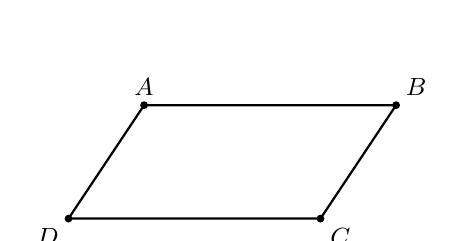
\begin{tikzpicture}[scale=0.8, font=\small]
  \coordinate (D) at (0,0);
  \coordinate (C) at (4,0);
  \coordinate (B) at (5.2,1.8);
  \coordinate (A) at (1.2,1.8);
  \draw[thick] (A) -- (B) -- (C) -- (D) -- cycle;
  \filldraw (A) circle (1.5pt) node[above] {$A$};
  \filldraw (B) circle (1.5pt) node[above right] {$B$};
  \filldraw (C) circle (1.5pt) node[below right] {$C$};
  \filldraw (D) circle (1.5pt) node[below left] {$D$};
\end{tikzpicture}
\end{center}
\choice
{$AB = CD, AD = BC$}
{$AB \parallel CD, AD \parallel BC$}
{\True $AB = BC = CD = DA$}
{Khẳng định A và B đều đúng}
\loigiai{
Hình bình hành có các cạnh đối song song và bằng nhau ($AB = CD, AD = BC$). Khẳng định $AB = BC = CD = DA$ chỉ đúng với hình thoi hoặc hình vuông, không đúng với hình bình hành tổng quát.
}
\end{ex}

\begin{ex}
Cho $x$ là ước của $24$ và $10 \le x < 15$. Vậy $x$ có giá trị bằng:
\choice
{\True $12$}
{$13$}
{$14$}
{$10$}
\loigiai{
Tập hợp các ước của 24 là $\{1; 2; 3; 4; 6; 8; 12; 24\}$. Giá trị thỏa mãn $10 \le x < 15$ là $x = 12$.
}
\end{ex}

\begin{ex}
Biểu diễn tập hợp $H = \{1; 2; 3; 4; 5\}$ bằng cách chỉ ra tính chất đặc trưng của nó là:
\choice
{$H = \{x \in \mathbb{N} \mid x \le 5\}$}
{$H = \{x \in \mathbb{N} \mid x < 5\}$}
{\True $H = \{x \in \mathbb{N}^* \mid x \le 5\}$}
{$H = \{x \in \mathbb{N}^* \mid x < 5\}$}
\loigiai{
Tập hợp $H$ gồm các số tự nhiên khác 0 nhỏ hơn hoặc bằng 5, viết là $H = \{x \in \mathbb{N}^* \mid x \le 5\}$.
}
\end{ex}

\begin{ex}
Trong các phân số sau, phân số nào là phân số tối giản?
\choice
{$\dfrac{26}{39}$}
{$\dfrac{15}{12}$}
{$\dfrac{27}{42}$}
{\True $\dfrac{3}{16}$}
\loigiai{
Ta có $\dfrac{26}{39} = \dfrac{2}{3}$; $\dfrac{15}{12} = \dfrac{5}{4}$; $\dfrac{27}{42} = \dfrac{9}{14}$. Phân số $\dfrac{3}{16}$ có tử số và mẫu số có ước chung lớn nhất bằng 1 nên là phân số tối giản.
}
\end{ex}

\begin{ex}
Số tự nhiên nào sau đây là ước của $12$?
\choice
{$0$}
{\True $4$}
{$5$}
{$10$}
\loigiai{
Vì $12 : 4 = 3$ nên 4 là ước của 12.
}
\end{ex}

\begin{ex}
Nêu cách đọc chuẩn của số $123\,875$:
\choice
{\True Một trăm hai mươi ba nghìn tám trăm bảy mươi lăm}
{Một hai ba nghìn tám bảy năm}
{Một trăm hai ba tám trăm bảy năm}
{Một trăm hai mươi ba nghìn bảy trăm tám mươi lăm}
\loigiai{
Số $123\,875$ đọc là: "Một trăm hai mươi ba nghìn tám trăm bảy mươi lăm" (hoặc Một trăm hai ba nghìn tám trăm bảy mươi lăm).
}
\end{ex}


\setcounter{ex}{0}
\vspace{2mm}
\noindent\textbf{\large PHẦN II. CÂU TRẮC NGHIỆM ĐÚNG SAI}
\vspace{1mm}
\begin{ex}
Cho biểu thức $M = 2^3 \cdot 3 - 5$. Xét tính đúng/sai của các khẳng định sau:
\choiceTF
{Giá trị của lũy thừa $2^3$ là $6$}
{Khi tính giá trị biểu thức $M$, ta thực hiện phép nhân trước, phép trừ sau}
{\True Giá trị của biểu thức $M$ là $19$}
{\True Giá trị của biểu thức $M$ là một số nguyên tố}
\loigiai{
\textbf{a)} Sai. Giá trị của lũy thừa $2^3$ là $2 \cdot 2 \cdot 2 = 8$.

\textbf{b)} Sai. Theo thứ tự thực hiện phép tính, ta phải tính lũy thừa trước, sau đó đến phép nhân, và cuối cùng mới thực hiện phép trừ.

\textbf{c)} Đúng. $M = 8 \cdot 3 - 5 = 24 - 5 = 19$.

\textbf{d)} Đúng. Số 19 lớn hơn 1 và chỉ có hai ước là 1 và 19 nên là số nguyên tố.
}
\end{ex}

\begin{ex}
Cho hình chữ nhật $ABCD$ có chiều dài $AB = 8\text{ cm}$ và chiều rộng $BC = 6\text{ cm}$. Xét tính đúng/sai của các khẳng định sau:
\choiceTF
{Bốn cạnh của hình chữ nhật $ABCD$ có độ dài bằng nhau}
{\True Các cạnh đối diện $AB$ và $CD$ song song và bằng nhau}
{Hai đường chéo $AC$ và $BD$ vuông góc với nhau}
{\True Chu vi của hình chữ nhật $ABCD$ là $28\text{ cm}$}
\loigiai{
\textbf{a)} Sai. Hình chữ nhật có các cạnh đối bằng nhau, không phải 4 cạnh bằng nhau.

\textbf{b)} Đúng. Trong hình chữ nhật, các cặp cạnh đối diện luôn song song và bằng nhau.

\textbf{c)} Sai. Hai đường chéo hình chữ nhật bằng nhau và cắt nhau tại trung điểm mỗi đường nhưng không vuông góc với nhau.

\textbf{d)} Đúng. Chu vi hình chữ nhật là $(8 + 6) \cdot 2 = 28\text{ (cm)}$.
}
\end{ex}


\setcounter{ex}{0}
\vspace{2mm}
\noindent\textbf{\large PHẦN III. CÂU HỎI TRẢ LỜI NGẮN}
\vspace{1mm}
\begin{ex}
Tìm các chữ số $x, y$ để số $\overline{35x98y}$ chia hết cho cả 2, 5 và 9. \shortans{x = 2, y = 0}
\loigiai{
Để $\overline{35x98y}$ chia hết cho cả 2 và 5 thì $y = 0$. Khi đó ta có số $\overline{35x980}$.\\Để số này chia hết cho 9 thì tổng các chữ số $(3 + 5 + x + 9 + 8 + 0) \ \vdots \ 9 \Rightarrow (25 + x) \ \vdots \ 9$. Vì $x$ là chữ số nên $x = 2$.\\Vậy $x = 2; y = 0$.
}
\end{ex}

\begin{ex}
Một hình thoi có độ dài hai đường chéo lần lượt là $8\text{ cm}$ và $10\text{ cm}$. Tính diện tích của hình thoi đó (theo đơn vị $\text{cm}^2$). \shortans{40}
\loigiai{
Diện tích hình thoi là: $S = \dfrac{8 \times 10}{2} = 40\text{ (cm}^2\text{)}$.
}
\end{ex}


\setcounter{ex}{0}
\vspace{2mm}
\noindent\textbf{\large PHẦN IV. TỰ LUẬN (BÀI TẬP VÀ BAREM ĐIỂM)}
\vspace{1mm}
\begin{ex} (1,0 điểm)
Thực hiện phép tính và tìm ước:
\begin{enumerate}[label=\textbf{\alph*)}, leftmargin=0.8cm, itemsep=2pt]
\item (0,5 điểm) Thực hiện phép tính: $6250 : \{50^2 : [112 - (32 - 2^2 \cdot 5)]\}$
\item (0,5 điểm) Tìm số tự nhiên $x \in Ư(30)$ thỏa mãn $x < 10$.
\end{enumerate}
\loigiai{
\textbf{a)} \textbf{[0,5 điểm]}\\ $6250 : \{2500 : [112 - (32 - 20)]\}\\= 6250 : \{2500 : [112 - 12]\}\\= 6250 : \{2500 : 100\}\\= 6250 : 25 = 250$.

\textbf{b)} \textbf{[0,5 điểm]}\\ Tập hợp các ước của 30 là: $Ư(30) = \{1; 2; 3; 5; 6; 10; 15; 30\}$.\\Vì $x < 10$ nên $x \in \{1; 2; 3; 5; 6\}$.


}
\end{ex}
\vspace{2mm}

\begin{ex} (1,0 điểm)
Phân tích các số sau ra thừa số nguyên tố:
\begin{enumerate}[label=\textbf{\alph*)}, leftmargin=0.8cm, itemsep=2pt]
\item (0,5 điểm) $60$
\item (0,5 điểm) $125$
\end{enumerate}
\loigiai{
\textbf{a)} \textbf{[0,5 điểm]}\\ $60 = 4 \cdot 15 = 2^2 \cdot 3 \cdot 5$.

\textbf{b)} \textbf{[0,5 điểm]}\\ $125 = 5^3$.


}
\end{ex}
\vspace{2mm}

\begin{ex} (1,0 điểm)
Bài toán hình học thực tế:
\begin{enumerate}[label=\textbf{\alph*)}, leftmargin=0.8cm, itemsep=2pt]
\item (0,5 điểm) Nêu các bước vẽ tam giác đều có độ dài cạnh bằng $3\text{ cm}$.
\item (0,5 điểm) Tính chu vi và diện tích mảnh đất có hình vẽ dưới đây:
\begin{center}
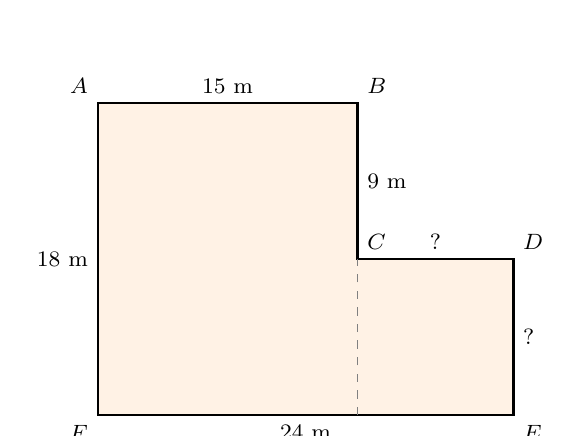
\begin{tikzpicture}[scale=0.22, font=\footnotesize]
  % Toa do cac dinh: A(0,18), B(15,18), C(15,9), D(24,9), E(24,0), F(0,0)
  \coordinate (F) at (0,0);
  \coordinate (A) at (0,18);
  \coordinate (B) at (15,18);
  \coordinate (C) at (15,9);
  \coordinate (D) at (24,9);
  \coordinate (E) at (24,0);
  \draw[thick, fill=orange!10] (A) -- (B) -- (C) -- (D) -- (E) -- (F) -- cycle;
  \draw[dashed, gray] (15,0) -- (15,9);
  \node[above] at (7.5,18) {$15\text{ m}$};
  \node[right] at (15,13.5) {$9\text{ m}$};
  \node[above] at (19.5,9) {$?$};
  \node[right] at (24,4.5) {$?$};
  \node[below] at (12,0) {$24\text{ m}$};
  \node[left] at (0,9) {$18\text{ m}$};
  \node[above left] at (A) {$A$};
  \node[above right] at (B) {$B$};
  \node[above right] at (C) {$C$};
  \node[above right] at (D) {$D$};
  \node[below right] at (E) {$E$};
  \node[below left] at (F) {$F$};
\end{tikzpicture}
\end{center}
\end{enumerate}
\loigiai{
\textbf{a)} \textbf{[0,5 điểm]}\\ \textbf{Cách vẽ tam giác đều cạnh $3\text{ cm}$:}
\begin{itemize}[leftmargin=1.5cm, topsep=1pt, itemsep=1pt]
  \item Vẽ đoạn thẳng $AB = 3\text{ cm}$.
  \item Dùng compa vẽ cung tròn tâm $A$ bán kính $3\text{ cm}$ và cung tròn tâm $B$ bán kính $3\text{ cm}$.
  \item Hai cung tròn cắt nhau tại điểm $C$.
  \item Nối $C$ với $A$ và $B$, ta được tam giác đều $ABC$ cạnh $3\text{ cm}$.
\end{itemize}
\begin{center}
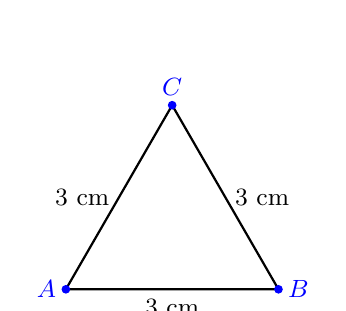
\begin{tikzpicture}[scale=0.9, font=\small]
  \coordinate (A) at (0,0);
  \coordinate (B) at (3,0);
  \coordinate (C) at (1.5, 2.598);
  \draw[thick] (A) -- (B) -- (C) -- cycle;
  \filldraw[blue] (A) circle (1.5pt) node[left] {$A$};
  \filldraw[blue] (B) circle (1.5pt) node[right] {$B$};
  \filldraw[blue] (C) circle (1.5pt) node[above] {$C$};
  \node[below] at (1.5,0) {$3\text{ cm}$};
  \node[left] at (0.75, 1.3) {$3\text{ cm}$};
  \node[right] at (2.25, 1.3) {$3\text{ cm}$};
\end{tikzpicture}
\end{center}

\textbf{b)} \textbf{[0,5 điểm]}\\ Độ dài hai cạnh còn thiếu là:\\$CD = 24 - 15 = 9\text{ (m)}$ và $DE = 18 - 9 = 9\text{ (m)}$.\\\textbf{Chu vi mảnh đất là:}\\$\mathcal{P} = 15 + 9 + 9 + 9 + 24 + 18 = 84\text{ (m)}$.\\\textbf{Diện tích mảnh đất là:}\\Chia mảnh đất thành hai hình chữ nhật: hình bên trái có kích thước $15\text{ m} \times 18\text{ m}$ và hình bên phải có kích thước $9\text{ m} \times 9\text{ m}$ (hoặc chia theo chiều ngang $15\text{ m} \times 9\text{ m}$ và $24\text{ m} \times 9\text{ m}$):\\$S = 15 \times 9 + 24 \times 9 = 135 + 216 = 351\text{ (m}^2\text{)}$.


}
\end{ex}
\vspace{2mm}


\begin{center}
\rule{4cm}{0.4pt}\\
\textit{--- HẾT ---}
\end{center}
\end{document}
